\documentclass[12pt]{article}
\usepackage{tikz}
\usepackage{pgfplots}
\pgfplotsset{compat=1.13}
\usepackage{pgfplotstable,filecontents}
\usepackage{csvsimple}


\usepackage{extsizes}
\usepackage{caption}
\usepackage{multirow}

\renewcommand{\epsilon}{\ensuremath{\varepsilon}}
\renewcommand{\phi}{\ensuremath{\varphi}}
\renewcommand{\kappa}{\ensuremath{\varkappa}}
\renewcommand{\le}{\ensuremath{\leqslant}}
\renewcommand{\leq}{\ensuremath{\leqslant}}
\renewcommand{\ge}{\ensuremath{\geqslant}}
\renewcommand{\geq}{\ensuremath{\geqslant}}
\renewcommand{\emptyset}{\varnothing}

\usepackage{geometry} % Простой способ задавать поля
\geometry{top=30mm}
\geometry{bottom=30mm}
\geometry{left=25mm}
\geometry{right=20mm}

\usepackage[T2A]{fontenc}			% кодировка
\usepackage[utf8]{inputenc}	
\usepackage[english,russian]{babel}   %% загружает пакет многоязыковой вёрстки
\usepackage{indentfirst}

\usepackage{amsmath,amsfonts,amssymb,amsthm,mathtools} 
\usepackage{graphicx}

\begin{document}
	\begin{minipage}{0.45\linewidth}
	Работу выполнил\\
	Самохин Валентин, 676 гр.\\[2mm]
	под руководством\\
	Артанова А.\,А\,.
	\end{minipage}
	\hfill
	\begin{minipage}{0.45\linewidth}\flushright
		Маршрут~IX \ №~8\\[3mm]
		12~апреля 2017~г.,\\
		\end{minipage}
		
		\vspace{8mm}
		\begin{center}
			\textbf{\Large Лабораторная работа №~2.2.1:}\\[\parskip]
			\LARGE Исследование взаимной диффузии газов
			\end{center}
			\vspace{0mm}
			
			\paragraph{Цель работы:}
			\begin{enumerate}
				\item регистрация зависимости концентрации гелия в воздухе от времени с помощью датчиков теплопроводности при разных начальных двалениях смеси газов;
				\item определение коэффициента диффузии по результатам измерений.
			\end{enumerate}
			
			\paragraph{В работе используются:}
			измерительная установка; форвакуумный насос; баллон с газом (гелий); манометр; источник питания; магазин сопротивлений .
			
			
			\vspace{2\parskip}
		\paragraph{Теоретическая справка.}
		В двухкомпонентной системе плотность потока вещества любого компонента в
		результате взаимной диффузии определяется законом Фика:
		\begin{equation}
		j_i = -D_{ij} \dfrac{\delta n_i}{\delta x},
		\end{equation}
		причём $D_{ij} = D_{ji} \equiv D$~--- коэффициент взаимной диффузии
		компонентов.
		
		Пусть два сосуда с объёмами $V_1, V_2$ соединены трубкой длины~$l$, сечения~$S$
		и заполнены смесью двух газов при одинаковом давлении (чтобы исключить
		макроскопические течения), но с разной концентрацией компонентов, причём один
		из компонентов преобладает.
		Вследствие взаимной диффузии концентрации каждого из компонентов со временем
		выравниваются, однако удобно рассматривать только концентрацию
		\emph{<<примеси>>.}
		
		Будем исходить из того, что описанный процесс происходит в основном благодаря
		диффузии в трубке, и считать процесс установления квазистационарным, тогда
		\begin{equation}
		J = -DS \frac{n_1 - n_2}{l},
		\end{equation}
		где $n_i$~--- концентрация примеси в $i$-ом сосуде. С учётом сохранения
		вещества запишем
		\begin{align}
		\dfrac{d(n_1 - n_2)}{dt} = -\frac{n_1 - n_2}{l} DS \left(\frac{1}{V_1} +
		\frac{1}{V_2}\right)
		&\Rightarrow
		\Delta n \equiv n_1 - n_2 = \Delta n_0 \exp\left(-\frac{t}{\tau}\right),
		\\		
		\tau \equiv \frac{V_1 V_2}{V_1 + V_2}& \frac{l}{SD}.
		\end{align}
		
		Для измерения концентраций будем применять датчики теплопроводности, считая
		линейными зависимость сопротивления от температуры и коэффициента
		теплопроводности от разности концентрации (раскладывая по Тейлору до первого члена, такой точности в нашем опыте достаточно).
		
		\paragraph{Экспериментальная установка}
		\subparagraph{Устройство установки:}V - сосуды, М - манометр, Т - выключатель, П.Б. - предохранительный баллон, Ф.Н. - форвакуумный насос, D - датчики теплопроводности.
		\begin{figure}[h]
				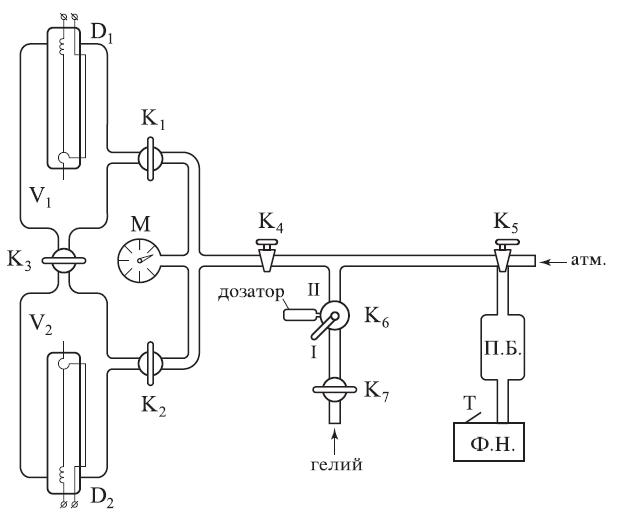
\includegraphics{1}
				\caption{Устройство установки}
		\end{figure}
		
		\begin{minipage}{0.45\textwidth}
			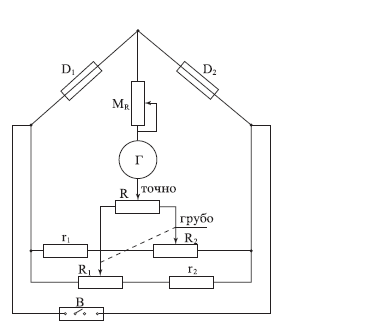
\includegraphics{2}
			\captionof{figure}{Устройство моста}
		\end{minipage}
		\hspace{1cm}
		\begin{minipage}{0.45\textwidth}
			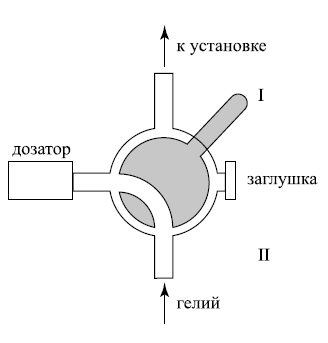
\includegraphics{3}
			\captionof{figure}{Кран К6}
		\end{minipage}
		\\
		Методика эксперимента заключается в том, что разность теплопроводностей изменяется пропорционально разности концентраций. Таким образом, показания гальванометра должны в процессе диффузии убывать по экспоненциальному закону, и установив зависимость показаний во времени, можно найти характерное время $\tau$, а из него коэффициент диффузии.	
		
		\section*{Выполнение работы}
		
		Измерениям предшествовали калибровка моста, сложный процесс закачки газов в объемы $V_1$ и $V_2$, ход которых не влияет на обработку результатов. Как было сказано ранее, замерив зависимость напряжения от времени, а затем прологарифмировав полученные значения, мы, из теории, должны были получить прямую. По ее коэффициенту наклона можно вычислить интересующие нас значения коэффициента диффузии, оценить размер частиц и длину свободного пробега.
		
		
		\begin{minipage}{0.3\textwidth}
		
			\pgfplotstabletypeset[
				col sep = semicolon,
				string type,
				every head row/.style={before row = {\hline}, after row = {\hline}},
				every last row/.style = {after row = {\hline}},
				every first column/.style ={
					column type/.add={|}{}},
				every last column/.style ={
					column type/.add={}{|}},
				columns/t/.style={column name = $t (c)$, column type = {|c}},
				columns/U/.style={column name = $U \textit{(мв)}$, column type = {|c|}},
				columns/l/.style={column name = $\ln U_0/U$, column type = {c|}},	
				]{40.csv}
		\captionof{table}{Показания при рабочем давлении 40 тор}	
	\end{minipage}	
	\hspace{2mm}	
	\begin{minipage}{0.6\textwidth}
			\pgfplotstabletypeset[
			col sep = semicolon,
			string type,
			every head row/.style={before row = {\hline}, after row = {\hline}},
			every last row/.style = {after row = {\hline}},
			every first column/.style ={
				column type/.add={|}{}},
			every last column/.style ={
				column type/.add={}{|}},
			columns/t/.style={column name = $t (c)$, column type = {|c}},
			columns/U/.style={column name = $U \textit{(мв)}$, column type = {|c|}},
			columns/l/.style={column name = $\ln U_0/U$, column type = {c|}},	
			]{104_1.txt}	
			\pgfplotstabletypeset[
			col sep = semicolon,
			string type,
			every head row/.style={before row = {\hline}, after row = {\hline}},
			every last row/.style = {after row = {\hline}},
			every first column/.style ={
				column type/.add={|}{}},
			every last column/.style ={
				column type/.add={}{|}},
			columns/t/.style={column name = $t (c)$, column type = {|c}},
			columns/U/.style={column name = $U \textit{(мв)}$, column type = {|c|}},
			columns/l/.style={column name = $\ln U_0/U$, column type = {c|}},	
			]{104_2.txt}
			\captionof{table}{Показания при рабочем давлении 104 тор}
			\end{minipage}	

		\begin{minipage}{0.6\textwidth}		
			\pgfplotstabletypeset[
			col sep = semicolon,
			string type,
			every head row/.style={before row = {\hline}, after row = {\hline}},
			every last row/.style = {after row = {\hline}},
			every first column/.style ={
				column type/.add={|}{}},
			every last column/.style ={
				column type/.add={}{|}},
			columns/t/.style={column name = $t (c)$, column type = {|c}},
			columns/U/.style={column name = $U \textit{(мв)}$, column type = {|c|}},
			columns/l/.style={column name = $\ln U_0/U$, column type = {c|}},	
			]{150_1.txt}
			\pgfplotstabletypeset[
			col sep = semicolon,
			string type,
			every head row/.style={before row = {\hline}, after row = {\hline}},
			every last row/.style = {after row = {\hline}},
			every first column/.style ={
				column type/.add={|}{}},
			every last column/.style ={
				column type/.add={}{|}},
			columns/t/.style={column name = $t (c)$, column type = {|c}},
			columns/U/.style={column name = $U \textit{(мв)}$, column type = {|c|}},
			columns/l/.style={column name = $\ln U_0/U$, column type = {c|}},	
			]{150_2.txt}
\captionof{table}{Показания при рабочем давлении 150 тор}
\end{minipage}
\hspace{0.5cm}
\begin{minipage}{0.3\textwidth}
	\pgfplotstabletypeset[
	col sep = semicolon,
	string type,
	every head row/.style={before row = {\hline}, after row = {\hline}},
	every last row/.style = {after row = {\hline}},
	every first column/.style ={
		column type/.add={|}{}},
		every last column/.style ={
			column type/.add={}{|}},
			columns/t/.style={column name = $t (c)$, column type = {|c}},
			columns/U/.style={column name = $U \textit{(мв)}$, column type = {|c|}},
			columns/l/.style={column name = $\ln U_0/U$, column type = {c|}},	
			]{last.csv}
			\captionof{table}{Показания при изменении долей газов}
			\end{minipage}	

\begin{minipage}{\textwidth}
	\centering
			\pgfplotstabletypeset[
			col sep = semicolon,
			string type,
			every head row/.style={before row = {\hline}, after row = {\hline}},
			every last row/.style = {after row = {\hline}},
			every first column/.style ={
				column type/.add={|}{}},
			every last column/.style ={
				column type/.add={}{|}},
			columns/t/.style={column name = $t (c)$, column type = {|c}},
			columns/U/.style={column name = $U \textit{(мв)}$, column type = {|c|}},
			columns/l/.style={column name = $\ln U_0/U$, column type = {c|}},	
			]{200_1.txt}
			\pgfplotstabletypeset[
			col sep = semicolon,
			string type,
			every head row/.style={before row = {\hline}, after row = {\hline}},
			every last row/.style = {after row = {\hline}},
			every first column/.style ={
				column type/.add={|}{}},
			every last column/.style ={
				column type/.add={}{|}},
			columns/t/.style={column name = $t (c)$, column type = {|c}},
			columns/U/.style={column name = $U \textit{(мв)}$, column type = {|c|}},
			columns/l/.style={column name = $\ln U_0/U$, column type = {c|}},	
			]{200_2.txt}
			\pgfplotstabletypeset[
			col sep = semicolon,
			string type,
			every head row/.style={before row = {\hline}, after row = {\hline}},
			every last row/.style = {after row = {\hline}},
			every first column/.style ={
				column type/.add={|}{}},
			every last column/.style ={
				column type/.add={}{|}},
			columns/t/.style={column name = $t (c)$, column type = {|c}},
			columns/U/.style={column name = $U \textit{(мв)}$, column type = {|c|}},
			columns/l/.style={column name = $\ln U_0/U$, column type = {c|}},	
			]{200_3.txt}
			\captionof{table}{Показания при рабочем давлении 200 тор}
		\end{minipage}
		
		
		\newpage
		\noindent
		\begin{minipage}{0.5\textwidth}
			\begin{tikzpicture}
			\begin{axis}[xlabel=$t (c)$,ylabel=$\ln U_0/U \cdot 10^2$,  xmin = 0, ymin = 0, minor tick num = 3, grid = both]
			\addplot [color=blue, only marks, mark = x,  error bars/.cd,
				x dir=both, x explicit, y dir=both, y explicit] table[col sep = semicolon, y index = 2, x index = 0] {data.csv};
			\addplot[domain = 0: 280, color = red]{0.121*x - 0.785};
			\end{axis}
			\end{tikzpicture}
			\captionof{figure}{График при $P = 40$ тор}
		\end{minipage}
		\hspace{0.5cm}
		\begin{minipage}{0.5\textwidth}
			\centering 
			$y=0,121x - 0,785$\\
			$1/\tau = 0,121$\\
			$M = (0,440 \pm 0,002) \textit{м}^2$\\
			$D = \dfrac{1}{\tau M}$\\
			$D = (0,281 \pm 0,007)10^{-2} \textit{м}^2/c$
		\end{minipage}
		\vspace{2cm}
		
		\noindent
		\begin{minipage}{0.5\textwidth}
			\begin{tikzpicture}
			\begin{axis}[xlabel=$t (c)$,ylabel=$\ln U_0/U \cdot 10^2$,  xmin = 0, ymin = 0, minor tick num = 3, grid = both]
			\addplot [color=blue, only marks, mark = x, error bars/.cd,
			x dir=both, x explicit, y dir=both, y explicit] table[col sep = semicolon, y index = 5, x index = 3] {data.csv};
			\addplot[domain = 0: 500, color = red]{0.0386*x + 0.1399};
			\end{axis}
			\end{tikzpicture}
			\captionof{figure}{График при $P = 104$ тор}
		\end{minipage}
		\hspace{0.5cm}
		\begin{minipage}{0.5\textwidth}
			\centering 
			$y=0,0386x - 0,1399$\\
			$1/\tau = 0,0386$\\
			$M = (0,440 \pm 0,002) \textit{м}^2$\\
			$D = \dfrac{1}{\tau M}$\\
			$D = (0,087 \pm 0,001)10^{-2} \textit{м}^2/c $
		\end{minipage}
		\vspace{2cm}
		\begin{minipage}{0.5\textwidth}
			\begin{tikzpicture}
			\begin{axis}[xlabel=$t (c)$,ylabel=$\ln U_0/U \cdot 10^2$,  xmin = 0, ymin = 0, minor tick num = 3, grid = both]
			\addplot [color=blue, mark = .,only marks,  error bars/.cd,
			x dir=both, x explicit, y dir=both, y explicit] table[col sep = semicolon, y index = 8, x index = 6, x error index = 15, y error index = 16] {data.csv};
			\addplot[domain = 0: 540, color = red]{0.0283*x + 0.0846};
			\end{axis}
			\end{tikzpicture}
			\captionof{figure}{График при $P = 150$ тор}
		\end{minipage}
		\hspace{0.5cm}
		\begin{minipage}{0.5\textwidth}
			\centering 
			$y=0,0283x + 0,0846$\\
			$1/\tau = 0,0283$\\
			$M = (0,440 \pm 0,002) \textit{м}^2$\\
			$D = \dfrac{1}{\tau M}$\\
			$D = (0,064 \pm 0,001)10^{-2} \textit{м}^2/c $
		\end{minipage}
		\vspace{2cm}
		\begin{minipage}{0.5\textwidth}
			\begin{tikzpicture}
			\begin{axis}[xlabel=$t (c)$,ylabel=$\ln U_0/U \cdot 10^2$,  xmin = 0, ymin = 0, minor tick num = 3, grid = both]
			\addplot [color=blue, mark = .,only marks,  error bars/.cd,
			x dir=both, x explicit, y dir=both, y explicit] table[col sep = semicolon, y index = 11, x index = 9, x error index = 15, y error index = 17] {data.csv};
			\addplot[domain = 0: 600, color = red]{0.0223*x + 0.0343};
			\end{axis}
			\end{tikzpicture}
			\captionof{figure}{График при $P = 200$ тор}
		\end{minipage}	
		\hspace{0.5cm}
		\begin{minipage}{0.5\textwidth}
			\centering 
			$y=0,0223x + 0,0343$\\
			$1/\tau = 0,0223$\\
			$M = (0,440 \pm 0,002) \textit{м}^2$\\
			$D = \dfrac{1}{\tau M}$\\
			$D = (0,051 \pm 0,001)10^{-2} \textit{м}^2/c $
		\end{minipage}
		\vspace{2cm}
		\begin{minipage}{0.5\textwidth}
			\begin{tikzpicture}
			\begin{axis}[xlabel=$t (c)$,ylabel=$\ln U_0/U \cdot 10^2$,  xmin = 0, ymin = 0, minor tick num = 3,  grid = both]
			\addplot [color=blue, mark = .,only marks,  error bars/.cd,
			x dir=both, x explicit, y dir=both, y explicit] table[col sep = semicolon, y index = 14, x index = 12, x error index = 15, y error index = 16] {data.csv};
			\addplot[domain = 0: 180, color = red]{0.1312*x + 0.0946};
			\end{axis}
			\end{tikzpicture}
			\captionof{figure}{График при $P = 40$ тор (при измененных пропорций)}
		\end{minipage}	
		\hspace{0.5cm}
		\begin{minipage}{0.5\textwidth}
			\centering 
			$y=0,1312x + 0,0946$\\
			$1/\tau = 0,0283$\\
			$M = (0,440 \pm 0,002) \textit{м}^2$\\
			$D = \dfrac{1}{\tau M}$\\
			$D = (0,298 \pm 0,005)10^{-2} \textit{м}^2/c $
		\end{minipage}
		\vspace{2cm}
		\begin{minipage}{0.5\textwidth}
			\begin{tikzpicture}
			\begin{axis}[xlabel={$1/P, \textit{тор}^{-1}$} , ylabel={$D, 10^{-2} \textit{м}^2/c$},  xmin = 0, ymin = 0, minor tick num = 3,  grid = both]
			\addplot [color=blue, mark = .,only marks,  error bars/.cd,
			x dir=both, x explicit, y dir=both, y explicit] table[col sep = semicolon, y index = 0, x index = 1, x error index = 3, y error index = 2] {extra.txt};
			\addplot[domain = 0.005: 0.025, color = red]{11.429*x - 0.0128};
			\end{axis}
			\end{tikzpicture}
			\captionof{figure}{График зависимости коэф. диффузии $D$ от $1/P$}
		\end{minipage}	
		\hspace{0.5cm}
		\begin{minipage}{0.5\textwidth}
			\centering 
			$y=11,429x - 0,0128$\\
			Экстраполяция даст:\\
			$D_{\textit{атм}} = (2,23 \pm 0,01) 10^{-5} \textit{м}^2/c$		
			
		\end{minipage}
		
		
		Оценим длину свободного пробега $\lambda$ и размер молекулы $d$:
		
		\begin{equation*}
		\lambda = 3D\sqrt{\dfrac{\mu}{3RT}} = (4,17 \pm 0,03) 10^{-7} \textit{м} 
		\end{equation*}
		
		\begin{equation*}
		d = \sqrt{\dfrac{kT}{P\lambda}} \sim 10^{-10} \textit{м} 
		\end{equation*}	
		
		\section*{Вывод}
		\begin{enumerate}
			\item Во-первых, по данным хорошо видно, что коэффициент взаимной диффузии газов не зависит от их пропорций (первый и последний опыты).
			\item Во-вторых, последний график недостаточно хорош. Видно, что не все точки лежат на прямой, что связано с плохой работой компьютера, использовавшегося с первых опытах.
			\item Наконец, оценка, произведенная в конце работы для размеров молекул, верна, что может говорить об относительно достоверных результатах.
		\end{enumerate}
		
\end{document}	